\section*{Conceitos Básicos}	
A forma de cálculos da HP-12C é pelo sistema RPN (\textit{Reverse Polish Notation}), no qual primeiro se digita o valor, informa sua entrada com a tecla \keystroke{$ENTER$}, digita o segundo valor e a tecla da função desejada. Segue-se esse raciocínio para todas as funções da calculadora, seja com a realização de operações básicas, financeiras ou de estatística; ou seja, primeiro digita-se os valores e por fim a função desejada. 
\begin{figure}[H]
	\centering
	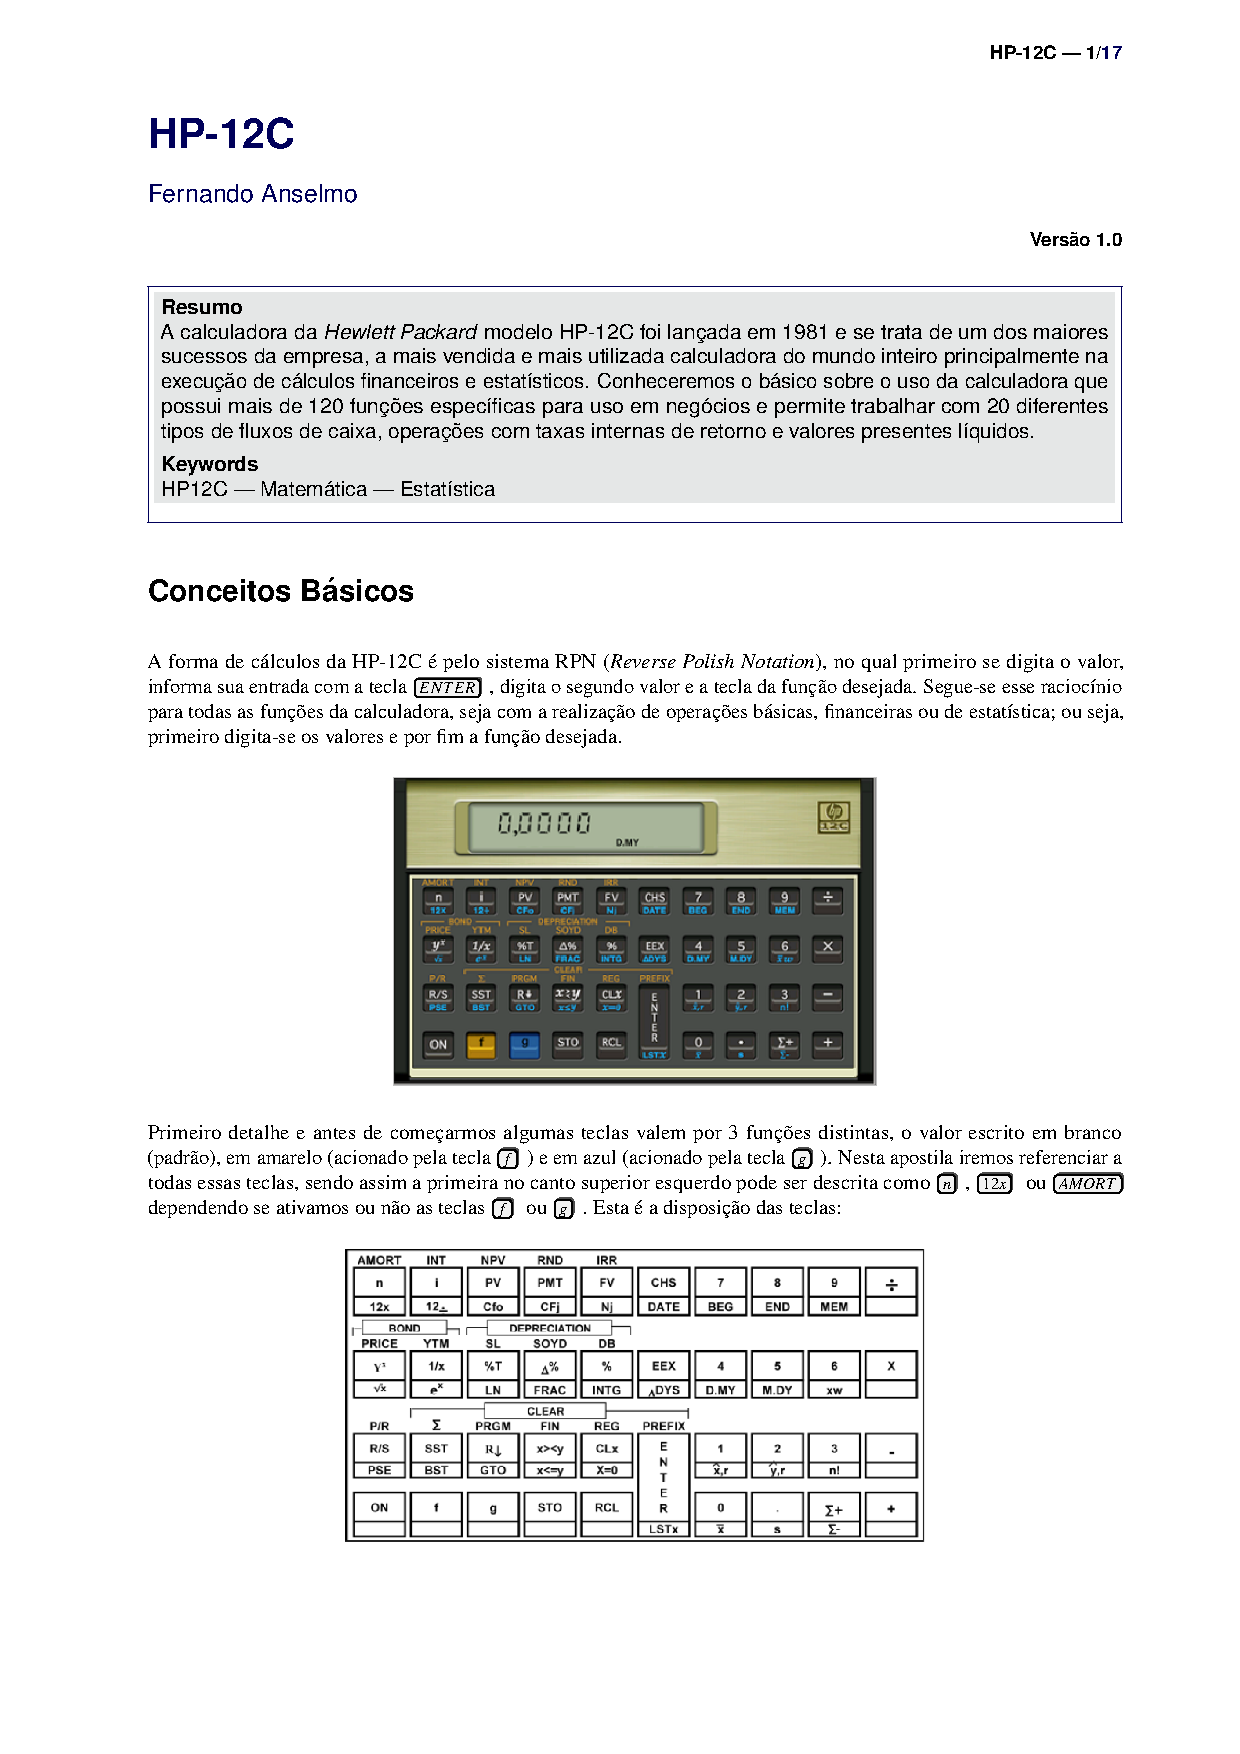
\includegraphics[width=0.5\textwidth]{images/hp12c}
\end{figure}
\vspace{-1em}
Primeiro detalhe e antes de começarmos algumas teclas valem por 3 funções distintas, o valor escrito em branco (padrão), em amarelo (acionado pela tecla \keystroke{$f$}) e em azul (acionado pela tecla \keystroke{$g$}). Nesta apostila iremos referenciar a todas essas teclas, sendo assim a primeira no canto superior esquerdo pode ser descrita como \keystroke{$n$}, \keystroke{$12x$} ou \keystroke{$AMORT$} dependendo se ativamos ou não as teclas \keystroke{$f$} ou \keystroke{$g$}. Esta é a disposição das teclas:
\begin{figure}[H]
	\centering
	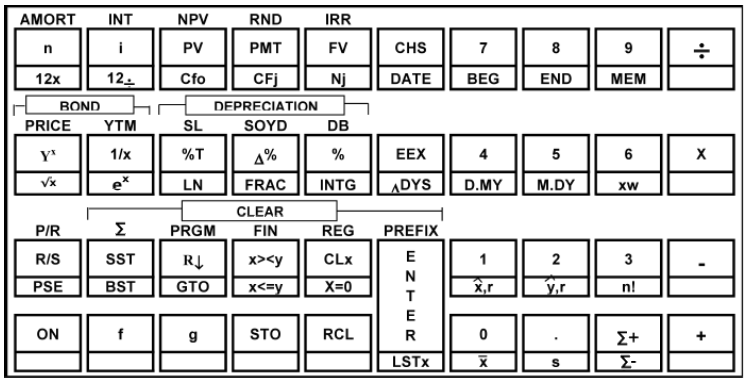
\includegraphics[width=0.6\textwidth]{images/teclado}
\end{figure}

\subsection*{Instalar a Calculadora}
Recomendo fortemente ter a máquina física, porém muitas pessoas possuem receio de comprarem e não se adaptarem, sendo assim podemos baixar uma versão \cite{hp12c} criada com a linguagem Java, testarmos todas as suas potencialidades e decidir.

Basta baixar o arquivo compactado, descompactar que na pasta gerada estão as instruções para seu uso, lembro que e assim como avisa o autor: "\textit{Este software foi desenvolvido para fins educacionais. \textbf{NÃO É RECOMENDADO} o uso deste para cálculos profissionais}".

\subsection*{Teste Inicial}
A calculadora possui alguns parâmetros que devemos conhecer, por exemplo, se ao ligar \keystroke{$ON$} aparecer no canto inferior esquerdo da tela um \textbf{*} isso indica que a bateria está fraca. O seguinte teste nos permite reconhecer se tudo está OK com seu funcionamento: \vspace{-1em}
\begin{enumerate}
	\item Desligar a calculadora
	\item Pressionar e segurar a tecla \keystroke{$\times$}
	\item Pressionar e soltar a tecla \keystroke{$ON$}
	\item Soltar a tecla \keystroke{$\times$}
\end{enumerate}

Aparecerá a palavra \textbf{RUNNING} piscando, em seguida todas as letras aparecerão (é ideal inclusive para saber se existe algum pixel queimado). Caso contrário será mostrado \textbf{ERRO}.

\subsection*{Códigos de Erro da HP-12C}
Estes são os códigos de erro que podem ser apresentados na calculadora devido a ações indevidas:
\begin{description}
	\item[Error 0] erro em operações matemáticas. Exemplos: divisão por zero, raiz quadrada com negativo, logaritmo com número menor ou igual a zero, fatorial com um não inteiro.
	\item[Error 1] ultrapassou a capacidade de armazenamento e processamento da máquina, isso é, a magnitude do resultado é igual ou superior a 10100. Por exemplo, fatorial de 73. Note que a mensagem de erro não aparece resulta apenas em uma série de noves no visor.
	\item[Error 2] operações estatísticas com erro. Por exemplo, média com n igual a 0.
	\item[Error 3] erro no cálculo da taxa interna de retorno (IRR). Neste caso, a mensagem informa que o cálculo é complexo, podendo envolver múltiplas respostas e não poderá prosseguir, a menos que você forneça uma estimativa para a taxa interna de retorno (IRR)
	\item[Error 4] erro em operações com a memória da calculadora. Por exemplo: tentativa na introdução com mais de 99 linhas para programação; ocorreu uma tentativa de desvio (GTO) para uma linha inexistente em um programa; tentativa de operação com os registradores de armazenamento (R5 a R9 ou R.0 a R.9); tentativa na utilização de um registrador ocupado com linha de programação.
	\item[Error 5] erro em operações com juros compostos. Provavelmente, algum valor foi colocado com o sinal errado (todos os valores têm o mesmo sinal), ou os valores para \keystroke{$i$}, \keystroke{$PV$} e \keystroke{$PF$} são tais, que não existe uma solução para \keystroke{$n$}.
	\item[Error 6] problemas no uso dos registradores de armazenamento. O registrador especificado não existe, ou foi convertido em linha de programação. Número para o fluxo de caixa foi superior a 20.
	\item[Error 7] problemas no cálculo da taxa interna de retorno (IRR). Não houve troca de sinal no fluxo de caixa.
	\item[Error 8] problemas com o calendário. Pode ser decorrente do emprego de data inapropriada ou em formato impróprio; tentativa na adição de dias além da capacidade.
	\item[Error 9] problemas no auto-teste. Ou o circuito da calculadora não está funcionando corretamente, ou algum procedimento no auto-teste apresentou falhas.
	\item[PR Error] perda irreparável da memória contínua.
\end{description}

\begin{theo}[Quanto a Problemas]{}
	Em caso de erros provavelmente a calculadora precisa de reparos ou não é original. O mais importante ressaltarmos que trata-se de uma máquina blindada, deste modo alguns problemas só seriam resolvidos com a troca desta.
\end{theo}

\subsection*{Bloquear e Desbloquear}
A calculadora pode ser bloqueada para impedir que outra pessoa sem conhecimento a utilize. Para bloquear pressionar as teclas \keystroke{$4$} \keystroke{$5$} \keystroke{$Enter$}, pressionar conjuntamente as teclas \keystroke{$ON$} \keystroke{$PMT$} e novamente em conjunto as teclas \keystroke{$ON$} \keystroke{$PMT$}, no visor aparece: \textbf{0.000000 45} e pressionar a tecla \keystroke{$1/x$}

Se tudo está correto agora a calculadora não liga mais, para desbloquear pressionar conjuntamente as teclas \keystroke{$ON$} \keystroke{$PMT$}

\subsection*{Limpeza}
Para deixar a calculadora da mesma forma como saiu de fábrica, siga os seguintes passos: \vspace{-1em}
\begin{enumerate}
	\item Desligar a calculadora
	\item Pressionar e segurar a tecla \keystroke{$-$}
	\item Pressionar e soltar a tecla \keystroke{$ON$}
	\item Soltar a tecla \keystroke{$-$}
\end{enumerate}

Ao término deve aparecer a mensagem: \textit{Pr Error}, caso contrário repita os passos até que a mensagem apareça. Para apagar os valores armazenados na calculadora utilizamos as seguintes teclas: \vspace{-1em}
\begin{itemize}
	\item \keystroke{$CLX$} - visor e registro de X (\textbf{CLear X}).
	\item \keystroke{$f$} \keystroke{$\sum$} - registradores estatísticos, pilhas e visor.
	\item \keystroke{$f$} \keystroke{$PRGM$} - memória de programação.
	\item \keystroke{$f$} \keystroke{$FIN$} - registros financeiros.
	\item \keystroke{$f$} \keystroke{$REG$} - registros (armazenamento de dados, financeiros, de pilha (LAST X) e visor).
\end{itemize}

\subsection*{Trabalhar com a Pilha}
A pilha operacional é um arquivo com 4 variáveis onde é possível armazenar dados para efetuar operações conjuntas, tais como fórmulas complexas, vejamos um exemplo:

Resolver a expressão: $(4,5 - 3,2) \div (8,4 - (1,3 \times 6))$

\keystroke{$4$} \keystroke{$.$} \keystroke{$5$} \keystroke{$Enter$} \keystroke{$3$} \keystroke{$.$} \keystroke{$2$} \keystroke{$-$} \keystroke{$8$} \keystroke{$.$} \keystroke{$4$} \keystroke{$Enter$} \keystroke{$1$} \keystroke{$.$} \keystroke{$3$} \keystroke{$Enter$} \keystroke{$6$} \keystroke{$\times$} \keystroke{$-$} \keystroke{$\div$}

Resultado \textbf{2,17}

\subsection*{Armazenar e Recuperar da Memória}
A calculadora possui 20 posições de memória definidas das teclas numéricas de 0 a 9 e .0 a .9, para armazenar em qualquer posição digitamos o número, pressionar a tecla \keystroke{$STO$} e indicar qual posição de memória. Para recuperar o valor pressionar a tecla \keystroke{$RCL$} e indicar qual posição de memória.

\subsection*{Mudanças}
Para realizar modificações na calculadora utilizamos as seguintes teclas: \vspace{-1em}
\begin{itemize}
	\item \keystroke{$ON$} \keystroke{$.$} -Alternar “.” ou “,” como separador decimal
	\item \keystroke{$CHS$} - Trocar o sinal de um número (\textit{CHange Sign})
	\item \keystroke{$f$} [núm] - Modificar a quantidade de casas decimais.
	\item \keystroke{$f$} \keystroke{$RND$} - Arredondar o número.
	\item \keystroke{$x \lessgtr y$} - Voltar para o último número digitado e incluído na máquina (corrigir valores).
	\item \keystroke{$R\downarrow$} - Troca os valores das Pilhas X, Y, Z e T (Roll down)
\end{itemize}

\subsection*{Lidar com Datas}
A calculadora permite trabalhar com datas entre 15/10/1582 a 25/11/4046. Para acertarmos a notação: \vspace{-1em}
\begin{itemize}
	\item \keystroke{$g$} \keystroke{$D.MY$} - Notação em D.MY (Europeia)
	\item \keystroke{$g$} \keystroke{$M.DY$} - Notação em M.DY (Americana)
\end{itemize}

Coloquemos em notação europeia (no visor aparece a informação na parte debaixo) e para introduzirmos a data 17/08/1966: \keystroke{$1$} \keystroke{$7$} \keystroke{$.$} \keystroke{$0$} \keystroke{$8$} \keystroke{$1$} \keystroke{$9$} \keystroke{$6$} \keystroke{$6$}

Temos na calculadora algumas funções que nos permite trabalhar com datas: \vspace{-1em}
\begin{itemize}
	\item data \keystroke{$Enter$} nDias \keystroke{$g$} \keystroke{$DATE$} - mostrar a próxima data
	\item data1 \keystroke{$Enter$} data2  \keystroke{$g$} \keystroke{$\bigtriangleup DYS$} - calcular a diferença entre duas datas
\end{itemize}	

\textbf{Problema 1}: Qual dia da semana cairá o Natal do ano 2021?

\keystroke{$2$} \keystroke{$5$} \keystroke{$.$} \keystroke{$1$} \keystroke{$2$} \keystroke{$2$} \keystroke{$0$} \keystroke{$2$} \keystroke{$1$} \keystroke{$Enter$} \keystroke{$0$} \keystroke{$g$} \keystroke{$DATE$}

Temos no visor o valor \textbf{25,12,2021 6}, que indica: 25/12/2021 Sexta\footnote{Valores para os dias da semana: 1-Seg 2-Ter 3-Qua 4-Qui 5-Sex 6-Sáb 7-Dom}

\textbf{Problema 2}: Em 09/05/2020 foi realizada uma aplicação em um banco para 90 dias. Qual a data de resgate e o dia da semana?

\keystroke{$0$} \keystroke{$9$} \keystroke{$.$} \keystroke{$0$} \keystroke{$5$} \keystroke{$2$} \keystroke{$0$} \keystroke{$2$} \keystroke{$0$} \keystroke{$Enter$} \keystroke{$9$} \keystroke{$0$} \keystroke{$g$} \keystroke{$DATE$}

Temos no visor o valor \textbf{8,08,2020 6}, que indica: 07/08/2020 Sexta

\textbf{Problema 3}: Uma aplicação por 90 dias foi resgatada no dia 07/08/2020. Qual foi o dia da aplicação?

\keystroke{$0$} \keystroke{$7$} \keystroke{$.$} \keystroke{$0$} \keystroke{$8$} \keystroke{$2$} \keystroke{$0$} \keystroke{$2$} \keystroke{$0$} \keystroke{$Enter$} \keystroke{$9$} \keystroke{$0$} \keystroke{$CHS$} \keystroke{$g$} \keystroke{$DATE$}

Temos no visor o valor \textbf{9,05,2020 6}, que indica: 09/05/2020 Sábado

\textbf{Problema 4}: Em 05/04/2020 foi aplicado dinheiro em um fundo de ações e o resgate do investimento em 15/08/2020. Qual o prazo real da aplicação e qual o número de dias entre as duas datas?

\keystroke{$0$} \keystroke{$5$} \keystroke{$.$} \keystroke{$0$} \keystroke{$4$} \keystroke{$2$} \keystroke{$0$} \keystroke{$2$} \keystroke{$0$} \keystroke{$Enter$} \keystroke{$1$} \keystroke{$5$} \keystroke{$.$} \keystroke{$0$} \keystroke{$8$} \keystroke{$2$} \keystroke{$0$} \keystroke{$2$} \keystroke{$0$} \keystroke{$g$} \keystroke{$\bigtriangleup DYS$}

A diferença é de \textbf{132} dias.
